

%% PSI AP Physics C
%%----------------------------------------


%% Dynamics
%%----------------------------------------
\element{njctl}{
\begin{question}{dynamics-q01}
    After firing a cannon ball,
        the cannon moves in the opposite direction from the ball.
    This an example of:
    \begin{choices}
        \wrongchoice{Newton's First Law}
        \wrongchoice{Newton's Second Law}
      \correctchoice{Newton's Third Law}
        \wrongchoice{Newton's Law of Gravitation}
        \wrongchoice{None of the provided}
    \end{choices}
\end{question}
}

\element{njctl}{
\begin{question}{dynamics-q02}
    In the absence of an external force a moving object will
    \begin{choices}
        \wrongchoice{slow down and come to a stop}
        \wrongchoice{speed up}
      \correctchoice{move with a constant speed in a straight line}
        \wrongchoice{turn to the right}
        \wrongchoice{turn to the left}
    \end{choices}
\end{question}
}

\element{njctl}{
\begin{question}{dynamics-q03}
    A loaded truck collides with a car causing a large amount of damage to the car.
    Which of the following is true about the collision?
    \begin{choices}
        \wrongchoice{The force on the truck is greater than the force on the car.}
        \wrongchoice{The force on the car is greater than the force on the truck.}
      \correctchoice{The force on the truck is the same in magnitude as the force on the car.}
        \wrongchoice{During the collision, the truck has a greater displacement than the car.}
        \wrongchoice{During the collision, the truck has a greater acceleration than the car.}
    \end{choices}
\end{question}
}

\element{njctl}{
\begin{question}{dynamics-q04}
    An object is thrown straight up.
    How do we compare the net force on the object to its weight when it is at the highest point in the path?
    \begin{choices}
        \wrongchoice{It is greater than the weight}
        \wrongchoice{It is slightly less than the weight}
        \wrongchoice{It is zero}
      \correctchoice{It is equal to the weight}
        \wrongchoice{It can't be determined}
    \end{choices}
\end{question}
}

\element{njctl}{
\begin{question}{dynamics-q05}
    An elevator car weighs \SI{5500}{\newton}.
    If the car accelerates upwards at a rate of \SI{4.0}{\meter\per\second\squared},
        what is the tension in the support cable lifting the car?
    Use $g=\SI{10}{\meter\per\second\squared}$.
    \begin{multicols}{2}
    \begin{choices}
        \wrongchoice{\SI{1600}{\newton}}
        \wrongchoice{\SI{3300}{\newton}}
        \wrongchoice{\SI{4400}{\newton}}
      \correctchoice{\SI{7700}{\newton}}
        \wrongchoice{\SI{8700}{\newton}}
    \end{choices}
    \end{multicols}
\end{question}
}

\newcommand{\njctlDynamicsQSix}{
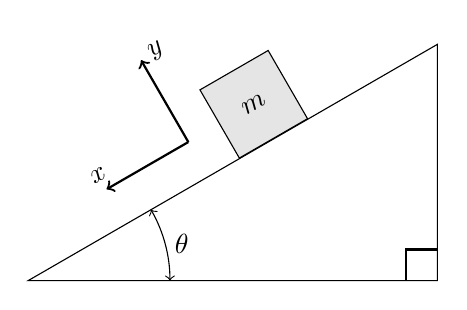
\begin{tikzpicture}[scale=1.2]
    %% Floor and plane
    \draw (0,0) -- (4.33,2.5) -- (4.33,0) -- cycle;
    \draw[thick] (4,0) -- (4,0.33) -- (4.33,0.33);
    %% angle
    \draw[<->] (1.5,0) arc(0:30:1.5) node[pos=0.5,anchor=west] {$\theta$};
    %% block
    \node[draw,minimum size=1cm,anchor=south,rotate=30,fill=white!90!black] (M) at (30:3) {$m$};
    %% Axis Lines
    \draw[thick,->] (M.center) ++(210:0.8) -- ++(210:1) node[anchor=south,rotate=30] {$x$};
    \draw[thick,->] (M.center) ++(210:0.8) -- ++(120:1) node[anchor=west,rotate=30] {$y$};
\end{tikzpicture}
}

\element{njctl}{
\begin{question}{dynamics-q06}
    The diagram below shows a block sliding down an incline plane.
    \begin{center}
        \njctlDynamicsQSix
    \end{center}
    Which of the following diagrams best represents the gravitational force $W$,
        the frictional force $f$, and the normal force $N$ that act on the block?
    \begin{multicols}{2}
    \begin{choices}
        \AMCboxDimensions{down=-1.5cm}
        \wrongchoice{
            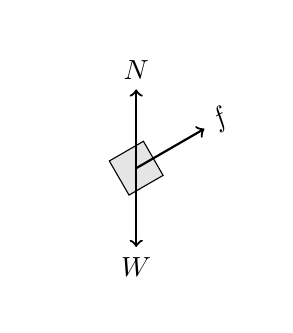
\begin{tikzpicture}[scale=0.5]
                \draw[white] (-3,-3) rectangle (3,4);
                \node[draw,fill=white!90!black,minimum size=0.5cm,rotate=30,anchor=south] (A) at (0,0) {};
                %\draw (210:2) -- (30:2);
                \draw[thick,->] (A.center) -- ++(90:2) node[anchor=south] {$N$};
                \draw[thick,->] (A.center) -- ++(270:2) node[anchor=north] {$W$};
                \draw[thick,->] (A.center) -- ++(30:2) node[anchor=west,rotate=30] {$f$};
            \end{tikzpicture}
        }
        \wrongchoice{
            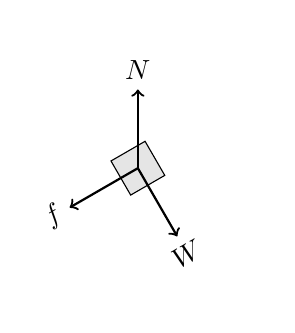
\begin{tikzpicture}[scale=0.5]
                \draw[white] (-3,-3) rectangle (3,4);
                \node[draw,fill=white!90!black,minimum size=0.5cm,rotate=30,anchor=south] (A) at (0,0) {};
                %\draw (210:2) -- (30:2);
                \draw[thick,->] (A.center) -- ++(90:2) node[anchor=south] {$N$};
                \draw[thick,->] (A.center) -- ++(300:2) node[anchor=north,rotate=30] {$W$};
                \draw[thick,->] (A.center) -- ++(210:2) node[anchor=east,rotate=30] {$f$};
            \end{tikzpicture}
        }
        %% ANS is C
        \correctchoice{
            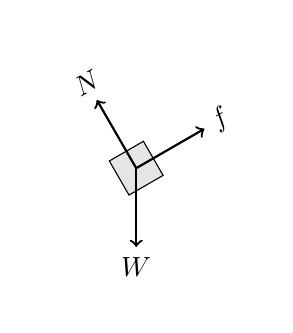
\begin{tikzpicture}[scale=0.5]
                \draw[white] (-3,-3) rectangle (3,4);
                \node[draw,fill=white!90!black,minimum size=0.5cm,rotate=30,anchor=south] (A) at (0,0) {};
                %\draw (210:2) -- (30:2);
                \draw[thick,->] (A.center) -- ++(120:2) node[anchor=south,rotate=30] {$N$};
                \draw[thick,->] (A.center) -- ++(270:2) node[anchor=north] {$W$};
                \draw[thick,->] (A.center) -- ++(30:2) node[anchor=west,rotate=30] {$f$};
            \end{tikzpicture}
        }
        \wrongchoice{
            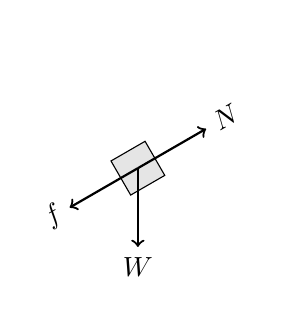
\begin{tikzpicture}[scale=0.5]
                \draw[white] (-3,-3) rectangle (3,4);
                \node[draw,fill=white!90!black,minimum size=0.5cm,rotate=30,anchor=south] (A) at (0,0) {};
                %\draw (210:2) -- (30:2);
                \draw[thick,->] (A.center) -- ++(30:2) node[anchor=west,rotate=30] {$N$};
                \draw[thick,->] (A.center) -- ++(270:2) node[anchor=north] {$W$};
                \draw[thick,->] (A.center) -- ++(210:2) node[anchor=east,rotate=30] {$f$};
            \end{tikzpicture}
        }
        \wrongchoice{
            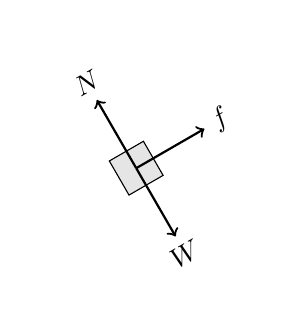
\begin{tikzpicture}[scale=0.5]
                \draw[white] (-3,-3) rectangle (3,4);
                \node[draw,fill=white!90!black,minimum size=0.5cm,rotate=30,anchor=south] (A) at (0,0) {};
                %\draw (210:2) -- (30:2);
                \draw[thick,->] (A.center) -- ++(120:2) node[anchor=south,rotate=30] {$N$};
                \draw[thick,->] (A.center) -- ++(300:2) node[anchor=north,rotate=30] {$W$};
                \draw[thick,->] (A.center) -- ++(30:2) node[anchor=west,rotate=30] {$f$};
            \end{tikzpicture}
        }
    \end{choices}
    \end{multicols}
\end{question}
}

\element{njctl}{
\begin{question}{dynamics-q07}
    A block with a mass $m=\SI{5}{\kilo\gram}$ slides down an inclined plane with an angle $\theta=\ang{37}$.
    The block maintains a constant acceleration $a=\SI{5.6}{\meter\per\second\squared}$.
    %% NOTE: is the digram actually needed?
    %% Could use \njctlDynamicsQSix, change theta to 37??
    The coefficient of kinetic friction between the block and the inclined surface is \num{0.05}.
    What is the normal force on the block by the inclined plane?
    ($\sin\ang{37}=0.6$, $\cos\ang{37}=0.8$).
    \begin{multicols}{3}
    \begin{choices}
        \wrongchoice{\SI{50}{\newton}}
      \correctchoice{\SI{40}{\newton}}
        \wrongchoice{\SI{30}{\newton}}
        \wrongchoice{\SI{20}{\newton}}
        \wrongchoice{\SI{10}{\newton}}
    \end{choices}
    \end{multicols}
\end{question}
}

\element{njctl}{
\begin{question}{dynamics-q08}
    A block with a mass $m=\SI{5}{\kilo\gram}$ slides down an inclined plane with an angle $\theta=\ang{37}$.
    The block maintains a constant acceleration $a=\SI{5.6}{\meter\per\second\squared}$.
    %% NOTE: is the digram actually needed?
    %% Could use \njctlDynamicsQSix, change theta to 37??
    The coefficient of kinetic friction between the block and the inclined surface is \num{0.05}.
    What is the friction force between the block and inclined plane?
    ($\sin\ang{37}=0.6$, $\cos\ang{37}=0.8$).
    \begin{multicols}{3}
    \begin{choices}
      \correctchoice{\SI{2}{\newton}}
        \wrongchoice{\SI{5}{\newton}}
        \wrongchoice{\SI{6}{\newton}}
        \wrongchoice{\SI{30}{\newton}}
        \wrongchoice{\SI{40}{\newton}}
    \end{choices}
    \end{multicols}
\end{question}
}

\element{njctl}{
\begin{question}{dynamics-q09}
    % NOTE: tikz
    %% This could be made better
    The coefficient of static friction between the block and the inclined plane is \num{0.4} and $\theta=\ang{25}$.
    The block is placed on the inclined plane.
    The block will:
    \begin{choices}
        \wrongchoice{not move.}
        \wrongchoice{start moving down the incline and then stop before it reaches the bottom of the incline.}
      \correctchoice{start moving down the incline and continue to increase its velocity.}
        \wrongchoice{start moving and increase its acceleration until it reaches the bottom of the incline.}
        \wrongchoice{start moving and then its acceleration will decrease.}
    \end{choices}
\end{question}
}

\element{njctl}{
\begin{question}{dynamics-q10}
    A system of two blocks is accelerated by an applied force of magnitude $F$ on the frictionless horizontal surface.
    \begin{center}
    \begin{tikzpicture}
        %% Ground
        \draw (-3,0) -- (3,0);
        \node[anchor=north,fill,pattern=north east lines,minimum width=6cm, minimum height=0.05cm] at (0,0) {};
        %% Blocks
        \node[draw,minimum size=1cm,anchor=south] (L) at (-2,0) {\SI{3}{\kilo\gram}};
        \node[draw,minimum size=1.2cm,anchor=south] (R) at (+1,0) {\SI{5}{\kilo\gram}};
        %% string and force
        \draw[thick] (R.west) -- ++(180:1.9cm);
        \draw[very thick,->] (R.east) -- ++(0:2cm) node[pos=0.5,anchor=south] {$F$};
    \end{tikzpicture}
    \end{center}
    The tension in the string between the blocks is:
    \begin{multicols}{3}
    \begin{choices}
        \wrongchoice{$3F$}
        \wrongchoice{$5F$}
      \correctchoice{$\dfrac{3F}{8}$}
        \wrongchoice{$\dfrac{F}{3}$}
        \wrongchoice{$\dfrac{F}{5}$}
    \end{choices}
    \end{multicols}
\end{question}
}

\element{njctl}{
\begin{question}{dynamics-q11}
    %% this is a duplicate of a halliday or serway question
    A student pulls a wooden box along a rough horizontal floor at constant speed by means of a force $P$ as shown to the right.
    \begin{center}
    \begin{tikzpicture}
        %% Ground
        \draw (-2,0) -- (2,0);
        \node[anchor=north,fill,pattern=north east lines,minimum width=4cm, minimum height=0.05cm] at (0,0) {};
        %% Blocks
        \node[draw,minimum size=1cm,anchor=south] (A) at (0,0) {};
        %% string and force
        \draw[thick,->] (A.center) -- ++(270:2cm) node[anchor=south west] {$W$};
        \draw[thick,->] (A.center) -- ++(180:2cm) node[anchor=south west] {$f$};
        \draw[thick,->] (A.center) -- ++(90:2cm) node[anchor=north west] {$N$};
        \draw[thick,->] (A.center) -- ++(30:2cm) node[anchor=south east] {$P$};
        \draw[dashed] (A.center) -- ++(0:2cm) node[pos=0.75,anchor=south] {$\theta$};
    \end{tikzpicture}
    \end{center}
    Which of the following must be true?
    \begin{multicols}{2}
    \begin{choices}
      \correctchoice{$P > f$ and $N < W$}
        \wrongchoice{$P > f$ and $N = W$}
        \wrongchoice{$P = f$ and $N > W$}
        \wrongchoice{$P = f$ and $N = W$}
        \wrongchoice{$P < f$ and $N = W$}
    \end{choices}
    \end{multicols}
\end{question}
}

\element{njctl}{
\begin{question}{dynamics-q12}
    As shown below,
        a boy pushes a sled of mass $m$ across a rough horizontal surface by applying a force of magnitude $F$ directed at an angle $\theta$.
    \begin{center}
    \begin{tikzpicture}
        %% Ground
        \draw (-3,0) -- (3,0);
        \node[anchor=north,fill,pattern=north east lines,minimum width=6cm, minimum height=0.05cm] at (0,0) {};
        %% mass
        \node[minimum size=1.5cm,draw,anchor=south] (M) at (+1,0) {$m$};
        %% force
        \draw[dashed] (M.west) -- ++(180:2);
        \draw[<->] (M.west) ++(180:1) arc(180:150:1) node[pos=0.5,anchor=east] {$\theta$};
        \draw[thick,<-] (M.west) ++(150:0.1) -- ++(150:2) node[pos=0.5,anchor=south,rotate=-30] {$F_{\text{app}}$};
    \end{tikzpicture}
    \end{center}
    The normal force on the sled is:
    \begin{multicols}{2}
    \begin{choices}
        \wrongchoice{$mg$}
        \wrongchoice{$mg\sin\theta$}
        \wrongchoice{$mg\cos\theta$}
      \correctchoice{$mg + F\sin\theta$}
        \wrongchoice{$mg - F\sin\theta$}
    \end{choices}
    \end{multicols}
\end{question}
}

\element{njctl}{
\begin{question}{dynamics-q13}
    A block of mass $m$ is pulled along a horizontal surface at constant speed $v$ by a force $F_{\text{app}}$,
        which acts at an angle of $\theta$ with the horizontal.
    \begin{center}
    \begin{tikzpicture}
        %% Ground
        \draw (-3,0) -- (3,0);
        \node[anchor=north,fill,pattern=north east lines,minimum width=6cm, minimum height=0.05cm] at (0,0) {};
        %% mass
        \node[minimum size=1.5cm,draw,anchor=south] (M) at (-1,0) {$m$};
        %% force
        \draw[dashed] (M.east) -- ++(0:2);
        \draw[<->] (M.east) ++(0:1) arc(0:30:1) node[pos=0.5,anchor=west] {$\theta$};
        \draw[thick,->] (M.east) -- ++(30:2) node[pos=0.5,anchor=south,rotate=30] {$F_{\text{app}}$};
    \end{tikzpicture}
    \end{center}
    The normal force exerted on the block by the surface is:
    \begin{multicols}{2}
    \begin{choices}
        \wrongchoice{$mg - F_{\text{app}}\cos\theta$}
      \correctchoice{$mg - F_{\text{app}}\sin\theta$}
        \wrongchoice{$mg$}
        \wrongchoice{$mg + F_{\text{app}}\sin\theta$}
        \wrongchoice{$mg + F_{\text{app}}\cos\theta$}
    \end{choices}
    \end{multicols}
\end{question}
}

\element{njctl}{
\begin{question}{dynamics-q14}
    An ideal spring obeys Hooke's law, $F=-kx$.
    A mass of \SI{0.30}{\kilo\gram} hung vertically from this spring stretches the spring 0.015 meter.
    The value of the spring constant is nearly:
    \begin{multicols}{3}
    \begin{choices}
        \wrongchoice{\SI{150}{\newton\per\meter}}
      \correctchoice{\SI{200}{\newton\per\meter}}
        \wrongchoice{\SI{300}{\newton\per\meter}}
        \wrongchoice{\SI{250}{\newton\per\meter}}
        \wrongchoice{\SI{350}{\newton\per\meter}}
    \end{choices}
    \end{multicols}
\end{question}
}

\element{njctl}{
\begin{question}{dynamics-q15}
    A block with a mass $m$ is placed on the top of an identical block $m$ and the system of two blocks is at rest on a rough horizontal surface as shown below.
    The top block is tied to the wall.
    The coefficient of static friction between all surfaces is $\mu_s$.
    \begin{center}
    \begin{tikzpicture}
        %% Ground
        \draw (0,0) -- (-6,0);
        \node[anchor=north,fill,pattern=north east lines,minimum width=6cm, minimum height=0.05cm] at (-3,0) {};
        %% Wall
        \draw (0,0) -- (0,3);
        \node[anchor=west,fill,pattern=north east lines,minimum width=0.1cm, minimum height=3.2cm] at (0,+1.4) {};
        %% block
        \node[fill=white!90!black,rounded corners=1ex,minimum width=2cm,minimum height=1cm,draw,anchor=south] (B) at (-3,0) {$m$};
        \node[fill=white!90!black,rounded corners=1ex,minimum width=2cm,minimum height=1cm,draw,anchor=south] (T) at (B.north) {$m$};
        %% force
        \draw[very thick,->] (B.west) -- ++(180:1.5) node[pos=0.5,anchor=south] {$F$};
        \draw[very thick] (T.east) -- ++(0:2);
    \end{tikzpicture}
    \end{center}
    What maximum value does force $F$ reach before the lower block starts sliding to the left?
    \begin{multicols}{3}
    \begin{choices}
      \correctchoice{$3\mu_s mg$}
        \wrongchoice{$2\mu_s mg$}
        \wrongchoice{$4\mu_s mg$}
        \wrongchoice{$\dfrac{\mu_s mg}{2}$}
        \wrongchoice{$\dfrac{\mu_s mg}{4}$}
    \end{choices}
    \end{multicols}
\end{question}
}

\element{njctl}{
\begin{question}{dynamics-q16}
    Three blocks connected with each other by two light strings.
    The blocks have different masses $m_2 > m_3 >m_1$.
    The heaviest of three blocks is placed on a frictionless table.
    \begin{center}
    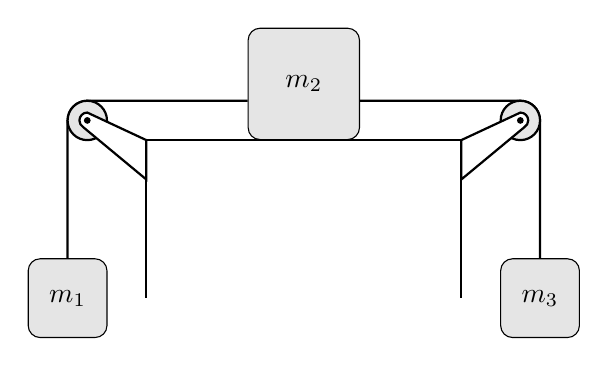
\begin{tikzpicture}
        %% Floor
        \draw[thick] (-2,-2) -- (-2,0) -- (2,0) -- (2,-2);
        %% Mass
        \node[draw,fill=white!90!black,rectangle,rounded corners=1ex,minimum size=1.414cm,anchor=south] (A) at (0,0) {$m_2$};
        \node[draw,fill=white!90!black,rectangle,rounded corners=1ex,minimum size=1.000cm,anchor=north] (B) at (3,-1.5) {$m_3$};
        \node[draw,fill=white!90!black,rectangle,rounded corners=1ex,minimum size=1.000cm,anchor=north] (C) at (-3,-1.5) {$m_1$};
        %% Rope
        \draw[thick] (A.south east) ++(90:0.5) -- (+2.75,0.5) arc(90:0:0.25) -- (B.north);
        \draw[thick] (A.south west) ++(90:0.5) -- (-2.75,0.5) arc(90:180:0.25) -- (C.north);
        %% Pully
        \draw[thick,fill=white!90!black] (+2.75,0.25) circle (0.25);
        \draw[thick,fill=white!90!black] (-2.75,0.25) circle (0.25);
        \draw[thick,fill=white] (2,0) -- (2.75,0.35) arc (90:-60:0.1) -- (2,-0.5) -- cycle;
        \draw[thick,fill=white] (-2,0) -- (-2.75,0.35) arc (90:240:0.1) -- (-2,-0.5) -- cycle;
        \draw[fill] (+2.75,0.25) circle (1pt);
        \draw[fill] (-2.75,0.25) circle (1pt);
    \end{tikzpicture}
    \end{center}
    The system of three blocks is released from rest.
    What is the acceleration of block $m_2$?
    \begin{multicols}{2}
    \begin{choices}
        \wrongchoice{$\dfrac{\left(m_2 - m_3 - m_1\right)g}{m_1 + m_2 + m_3}$}
        \wrongchoice{$\dfrac{\left(m_1 - m_3 - m_2\right)g}{m_1 + m_2 + m_3}$}
      \correctchoice{$\dfrac{\left(m_3 - m_1\right)g}{m_1 + m_2 + m_3}$}
        \wrongchoice{$\dfrac{\left(m_3 - m_2 - m_1\right)g}{m_1 + m_2 + m_3}$}
        \wrongchoice{$\dfrac{\left(m_1 - m_3\right)g}{m_1 + m_2 + m_3}$}
    \end{choices}
    \end{multicols}
\end{question}
}

\element{njctl}{
\begin{question}{dynamics-q17}
    A lamp of mass $m$ is suspended from two cables of unequal length as shown below.
    \begin{center}
    \begin{tikzpicture}
        %% NOTE: tikz
    \end{tikzpicture}
    \end{center}
    Which of the following is true about the tensions $T_1$ and $T_2$ in the cables?
    \begin{multicols}{2}
    \begin{choices}
        \wrongchoice{$T_1 > T_2$}
        \wrongchoice{$T_1 = T_2$}
      \correctchoice{$T_2 > T_1$}
        \wrongchoice{$T_1 - T_2 = mg$}
        \wrongchoice{$T_1 + T_2 = mg$}
    \end{choices}
    \end{multicols}
\end{question}
}

\element{njctl}{
\begin{question}{dynamics-q18}
    A ball of mass $m$ is suspended from two massless strings of an equal length as shown below.
    \begin{center}
    \begin{tikzpicture}
        %% NOTE: tikz
        %% Ceiling
        \node[anchor=south,fill,pattern=north east lines,minimum width=3cm, minimum height=0.05cm] at (0,0) {};
        \draw (-1.5,0) -- (1.5,0);
        %% mass
        \node[circle,minimum size=0.9cm,fill=white!90!black] (M) at (0,-3) {$m$};
        %% strings
        \draw[dashed] (0,0) -- (M.center);
        \draw (-2,0) -- (M.center);
        \draw (+2,0) -- (M.center);
        %% angles
        \draw[<->] (0,-1) arc(90:123:2) node[pos=0.5,anchor=south] {$\theta$};
        \draw[<->] (0,-1) arc(90:56:2) node[pos=0.5,anchor=south] {$\theta$};
    \end{tikzpicture}
    \end{center}
    The tension force in each string is:
    \begin{multicols}{2}
    \begin{choices}
        \wrongchoice{$\dfrac{mg\cos\theta}{2}$}
        \wrongchoice{$2mg\cos\theta$}
        \wrongchoice{$mg\cos\theta$}
        \wrongchoice{$\dfrac{mg}{\cos\theta}$}
      \correctchoice{$\dfrac{mg}{2\cos\theta}$}
    \end{choices}
    \end{multicols}
\end{question}
}

\element{njctl}{
\begin{question}{dynamics-q19}
    A ball moves horizontally with an initial velocity $v_0$, as shown below.
    \begin{center}
    \begin{tikzpicture}
        %% ball v
        \draw (0,0) circle (0.25cm);
        \draw[very thick,->] (0,0) -- (1.5,0) node[pos=0.5,anchor=south] {$v$};
        \draw[dashed] (1.5,0) -- (3,0);
        %% ball v_0
        \draw (0,-3) circle (0.25cm);
        \draw[very thick,->] (0,-3) -- (0,-1.5) node[pos=0.5,anchor=east] {$v_0$};
        \draw[dashed] (0,-1.5) -- (0,0);
    \end{tikzpicture}
    \end{center}
    It is then struck by a tennis racket.
    After leaving the racket, the ball moves with a velocity $v$.
    Which of the following vectors best represents the direction of the average force that the racket exerts on the ball?
    \begin{multicols}{3}
    \begin{choices}
        \AMCboxDimensions{down=-0.4cm}
        \wrongchoice{
            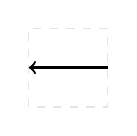
\begin{tikzpicture}
                \draw[dashed,white!90!black] (0,0) rectangle (1,1);
                \draw[thick,->] (1,0.5) -- (0,0.5);
            \end{tikzpicture}
        }
        \wrongchoice{
            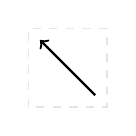
\begin{tikzpicture}
                \draw[dashed,white!90!black] (0,0) rectangle (1,1);
                \draw[thick,->] (0.85,0.15) -- (0.15,0.85);
            \end{tikzpicture}
        }
        \wrongchoice{
            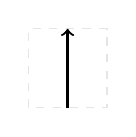
\begin{tikzpicture}
                \draw[dashed,white!90!black] (0,0) rectangle (1,1);
                \draw[thick,->] (0.5,0) -- (0.5,1);
            \end{tikzpicture}
        }
        %% ANS is D
        \correctchoice{
            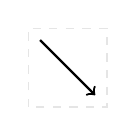
\begin{tikzpicture}
                \draw[dashed,white!90!black] (0,0) rectangle (1,1);
                \draw[thick,->] (0.15,0.85) -- (0.85,0.15);
            \end{tikzpicture}
        }
        \wrongchoice{
            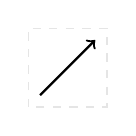
\begin{tikzpicture}
                \draw[dashed,white!90!black] (0,0) rectangle (1,1);
                \draw[thick,->] (0.15,0.15) -- (0.85,0.85);
            \end{tikzpicture}
        }
    \end{choices}
    \end{multicols}
\end{question}
}

\element{njctl}{
\begin{question}{dynamics-q20}
    A marble of mass $m$ moves along a path with a speed defined by the function $v = bt^2 + c$,
        where $t$ is time and $b$ and $c$ are constants.
    What is the magnitude $F$ of the net force on the particle at time $t = t_1$?
    \begin{multicols}{2}
    \begin{choices}
        \wrongchoice{$bt_1^2 + c$}
        \wrongchoice{$3mbt_1 + 2c$}
        \wrongchoice{$mbt_1$}
        \wrongchoice{$mbt_1 + c$}
      \correctchoice{$2mbt_1$}
    \end{choices}
    \end{multicols}
\end{question}
}

\element{njctl}{
\begin{question}{dynamics-q21}
    The position as a function of time of a moving object is given by the formula $x = 2t^3 - 3t^2 + 4t$.
    At what time is the net force on the object is zero?
    \begin{multicols}{3}
    \begin{choices}
      \correctchoice{\SI{0.5}{\second}}
        \wrongchoice{\SI{1.0}{\second}}
        \wrongchoice{\SI{1.5}{\second}}
        \wrongchoice{\SI{1.8}{\second}}
        \wrongchoice{\SI{2.2}{\second}}
    \end{choices}
    \end{multicols}
\end{question}
}

\element{njctl}{
\begin{question}{dynamics-q22}
    The velocity as a function of time of a moving object is shown by the graph.
    \begin{center}
    \begin{tikzpicture}
        \begin{axis}[
            axis y line=left,
            axis x line=bottom,
            axis line style={->},
            xlabel={time},
            xtick=\empty,
            ylabel={velocity},
            ytick=\empty,
            grid=major,
            xmin=0,xmax=11,
            ymin=0,ymax=11,
            width=0.8\columnwidth,
            height=0.5\columnwidth,
        ]
        \addplot[line width=1pt,domain=0:10]{0.1*x*x};
        \end{axis}
    \end{tikzpicture}
    \end{center}
    Which of the following graphs best represents the magnitude of the net force exerted on the object as a function of time?
    \begin{multicols}{2}
    \begin{choices}
        \AMCboxDimensions{down=-1.5em}
        \wrongchoice{
            \begin{tikzpicture}
                \begin{axis}[
                    axis y line=left,
                    axis x line=bottom,
                    axis line style={->},
                    xlabel={time},
                    xtick=\empty,
                    ylabel={force},
                    ytick=\empty,
                    grid=major,
                    xmin=0,xmax=11,
                    ymin=0,ymax=11,
                    width=0.95\columnwidth,
                ]
                \addplot[line width=1pt,domain=0:10]{3.15 * sqrt(x)};
                \end{axis}
            \end{tikzpicture}
        }
        \wrongchoice{
            \begin{tikzpicture}
                \begin{axis}[
                    axis y line=left,
                    axis x line=bottom,
                    axis line style={->},
                    xlabel={time},
                    xtick=\empty,
                    ylabel={force},
                    ytick=\empty,
                    grid=major,
                    xmin=0,xmax=11,
                    ymin=0,ymax=11,
                    width=0.95\columnwidth,
                ]
                \addplot[line width=1pt,domain=0:10]{0.1*x*x};
                \end{axis}
            \end{tikzpicture}
        }
        \wrongchoice{
            \begin{tikzpicture}
                \begin{axis}[
                    axis y line=left,
                    axis x line=bottom,
                    axis line style={->},
                    xlabel={time},
                    xtick=\empty,
                    ylabel={force},
                    ytick=\empty,
                    grid=major,
                    xmin=0,xmax=11,
                    ymin=0,ymax=11,
                    width=0.95\columnwidth,
                ]
                \addplot[line width=1pt,domain=0:10]{10-x};
                \end{axis}
            \end{tikzpicture}
        }
        \wrongchoice{
            \begin{tikzpicture}
                \begin{axis}[
                    axis y line=left,
                    axis x line=bottom,
                    axis line style={->},
                    xlabel={time},
                    xtick=\empty,
                    ylabel={force},
                    ytick=\empty,
                    grid=major,
                    xmin=0,xmax=11,
                    ymin=0,ymax=11,
                    width=0.95\columnwidth,
                ]
                \addplot[line width=1pt,domain=0:10]{8};
                \end{axis}
            \end{tikzpicture}
        }
        %% ANS is E
        \correctchoice{
            \begin{tikzpicture}
                \begin{axis}[
                    axis y line=left,
                    axis x line=bottom,
                    axis line style={->},
                    xlabel={time},
                    xtick=\empty,
                    ylabel={force},
                    ytick=\empty,
                    grid=major,
                    xmin=0,xmax=11,
                    ymin=0,ymax=11,
                    width=0.95\columnwidth,
                ]
                \addplot[line width=1pt,domain=0:10]{x};
                \end{axis}
            \end{tikzpicture}
        }
    \end{choices}
    \end{multicols}
\end{question}
}

\element{njctl}{
\begin{question}{dynamics-q23}
    A box of \SI{50}{\kilo\gram} is pulled up from rest by a cable.
    \begin{center}
    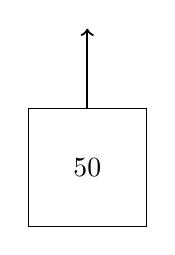
\begin{tikzpicture}
        \node[draw,minimum size=1.5cm] (A) at (0,0) {\SI{50}{\kilo\gram}};
        \draw[thick,->] (A.north) -- ++(90:1cm);
    \end{tikzpicture}
    \end{center}
    The tension force in the cable is \SI{600}{\newton}.
    What is the box's velocity after it covers vertical distance of \SI{16}{\meter}?
    \begin{multicols}{3}
    \begin{choices}
        \wrongchoice{\SI{4}{\meter\per\second}}
      \correctchoice{\SI{8}{\meter\per\second}}
        \wrongchoice{\SI{12}{\meter\per\second}}
        \wrongchoice{\SI{16}{\meter\per\second}}
        \wrongchoice{\SI{20}{\meter\per\second}}
    \end{choices}
    \end{multicols}
\end{question}
}

\element{njctl}{
\begin{question}{dynamics-q24}
    An Atwood machine is presented by the diagram.
    \begin{center}
    \begin{tikzpicture}
        %% Ceiling
        \node[anchor=south,fill,pattern=north east lines,minimum width=3cm, minimum height=0.05cm] at (0,0) {};
        \draw (-1.5,0) -- (1.5,0);
        %% Masses
        \node[draw,fill=white!90!black,rectangle,minimum size=1.00cm] (A) at (-0.80,-3) {\SI{0.50}{\kilo\gram}};
        \node[draw,fill=white!90!black,rectangle,minimum size=1.22cm] (B) at (+0.80,-4) {\SI{0.75}{\kilo\gram}};
        %% Rope
        \draw[thick] (A.north) -- (-0.80,-1.00) arc(180:0:0.80) -- (B.north);
        %% Pulley
        \draw[fill=white!90!black] (0,-1) circle (0.80);
        \draw[fill=white!60!black] (-0.25,0) -- (-0.15,-1.05) arc(190:350:0.15) -- (0.25,0) --cycle;
        \draw[fill] (0,-1) circle (1.5pt);
    \end{tikzpicture}
    \end{center}
    What is the magnitude of the acceleration for the \SI{0.5}{\kilo\gram} block?
    \begin{multicols}{3}
    \begin{choices}
        \wrongchoice{\SI{6}{\meter\per\second\squared}}
        \wrongchoice{\SI{4}{\meter\per\second\squared}}
      \correctchoice{\SI{2}{\meter\per\second\squared}}
        \wrongchoice{\SI{1}{\meter\per\second\squared}}
        \wrongchoice{\SI{0.5}{\meter\per\second\squared}}
    \end{choices}
    \end{multicols}
\end{question}
}

\newcommand{\njctlDynamicsQTwentyFive}{
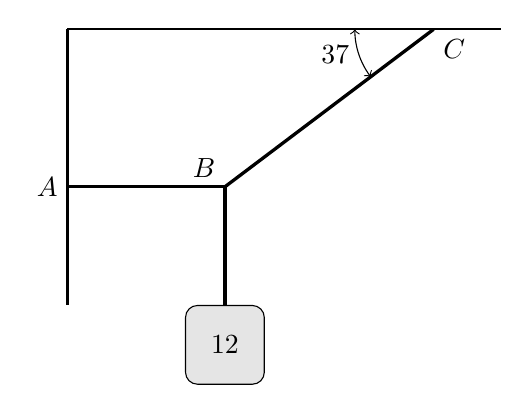
\begin{tikzpicture}
    %% NOTE: TODO: add pattern to wall and ceiling
    %% coordinates
    \coordinate (A) at (0,-2);
    \coordinate (B) at (2,-2);
    \coordinate (C) at (4.65,0);
    %% Nodes
    \node[anchor=east] at (A) {$A$};
    \node[anchor=south east] at (B) {$B$};
    \node[anchor=north west] at (C) {$C$};
    %% Lines
    \draw[thick] (0,0) -- (5.5,0);
    \draw[thick] (0,0) -- (0,-3.5);
    \draw[very thick] (A) --  (B);
    \draw[very thick] (B) --  (C);
    %% angle
    \draw[<->] (C) ++(180:1) arc (180:217:1) node[pos=0.5,anchor=east] {\ang{37}};
    %% Mass
    \node[draw,fill=white!90!black,rectangle,rounded corners=1ex,minimum size=1cm,anchor=north,yshift=-0.5cm] (M) at (2,-3) {\SI{12}{\kilo\gram}};
    \draw[very thick] (M.north) -- (B);
\end{tikzpicture}
}

\element{njctl}{
\begin{question}{dynamics-q25}
    A \SI{12}{\kilo\gram} sphere is supported by two ropes $AB$ and $BC$.
    \begin{center}
        \njctlDynamicsQTwentyFive
    \end{center}
    What is the tension force in rope $BC$?
    \begin{multicols}{3}
    \begin{choices}
        \wrongchoice{\SI{120}{\newton}}
        \wrongchoice{\SI{160}{\newton}}
        \wrongchoice{\SI{180}{\newton}}
      \correctchoice{\SI{200}{\newton}}
        \wrongchoice{\SI{240}{\newton}}
    \end{choices}
    \end{multicols}
\end{question}
}

\element{njctl}{
\begin{question}{dynamics-q26}
    A \SI{12}{\kilo\gram} sphere is supported by two ropes $AB$ and $BC$.
    \begin{center}
        \njctlDynamicsQTwentyFive
    \end{center}
    What is the tension force in rope $AB$?
    \begin{multicols}{3}
    \begin{choices}
        \wrongchoice{\SI{120}{\newton}}
      \correctchoice{\SI{160}{\newton}}
        \wrongchoice{\SI{180}{\newton}}
        \wrongchoice{\SI{200}{\newton}}
        \wrongchoice{\SI{240}{\newton}}
    \end{choices}
    \end{multicols}
\end{question}
}

\element{njctl}{
\begin{question}{dynamics-q27}
    A small sphere is attached to a light string that can move in a vertical circle.
    The sphere is released from point 1 and describes a semicircle when it reaches point 2.
    \begin{center}
    \begin{tikzpicture}
        \draw[dashed] (0,0) circle (2cm);
        \draw (0,0) -- (180:2);
        \draw (0,0) -- (270:2);
        \draw[fill] (180:2) circle (5pt) node[xshift=-5pt,anchor=east] {$1$};
        \draw[fill] (270:2) circle (5pt) node[yshift=-5pt,anchor=north] {$2$};
    \end{tikzpicture}
    \end{center}
    What are the directions of the acceleration vector at point 1 and point 2?
    \begin{choices}
        %% NOTE: Table options
      \correctchoice{Downward Upward}
        \wrongchoice{Downward To the right}
        \wrongchoice{Upward Upward}
        \wrongchoice{To the right Upward}
        \wrongchoice{To the right Downward}
    \end{choices}
\end{question}
}

\element{njctl}{
\begin{question}{dynamics-q28}
    A particle moves along a curved path from point 1 to point 2.
    Which of the following diagrams indicates a possible combination of the net force,
        acceleration and velocity of the particle?
    \begin{multicols}{2}
    \begin{choices}
        \AMCboxDimensions{down=-1cm}
        \wrongchoice{
            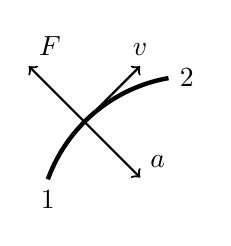
\begin{tikzpicture}
                %% path
                \draw[ultra thick] (160:2) arc (160:100:2)
                    node[pos=0,anchor=north] {$1$}
                    node[pos=1,anchor=west] {$2$};
                %% vectors
                \draw[thick,->] (135:2) -- ++(45:1) node[anchor=south] {$v$};
                \draw[thick,->] (135:2) -- ++(135:1) node[anchor=south west] {$F$};
                \draw[thick,->] (135:2) -- ++(315:1) node[anchor=south west] {$a$};
            \end{tikzpicture}
        }
        \wrongchoice{
            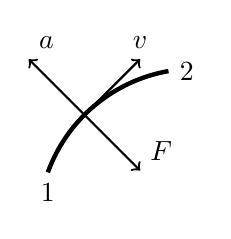
\begin{tikzpicture}
                %% path
                \draw[ultra thick] (160:2) arc (160:100:2)
                    node[pos=0,anchor=north] {$1$}
                    node[pos=1,anchor=west] {$2$};
                %% vectors
                \draw[thick,->] (135:2) -- ++(45:1) node[anchor=south] {$v$};
                \draw[thick,->] (135:2) -- ++(135:1) node[anchor=south west] {$a$};
                \draw[thick,->] (135:2) -- ++(315:1) node[anchor=south west] {$F$};
            \end{tikzpicture}
        }
        \wrongchoice{
            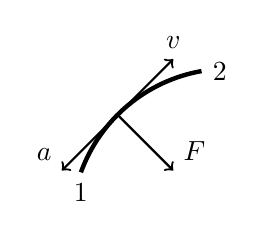
\begin{tikzpicture}
                %% path
                \draw[ultra thick] (160:2) arc (160:100:2)
                    node[pos=0,anchor=north] {$1$}
                    node[pos=1,anchor=west] {$2$};
                %% vectors
                \draw[thick,->] (135:2) -- ++(45:1) node[anchor=south] {$v$};
                \draw[thick,->] (135:2) -- ++(225:1) node[anchor=south east] {$a$};
                \draw[thick,->] (135:2) -- ++(315:1) node[anchor=south west] {$F$};
            \end{tikzpicture}
        }
        \wrongchoice{
            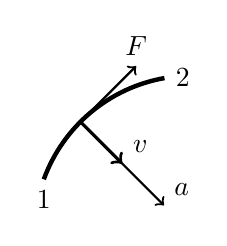
\begin{tikzpicture}
                %% path
                \draw[ultra thick] (160:2) arc (160:100:2)
                    node[pos=0,anchor=north] {$1$}
                    node[pos=1,anchor=west] {$2$};
                %% vectors
                \draw[thick,->] (135:2) -- ++(45:1) node[anchor=south] {$F$};
                \draw[very thick,->] (135:2) -- ++(315:0.75) node[anchor=south west] {$v$};
                \draw[thick,->] (135:2) -- ++(315:1.5) node[anchor=south west] {$a$};
            \end{tikzpicture}
        }
        %% NOTE: ANS is E
        \correctchoice{
            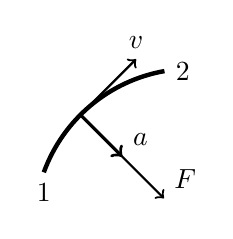
\begin{tikzpicture}
                %% path
                \draw[ultra thick] (160:2) arc (160:100:2)
                    node[pos=0,anchor=north] {$1$}
                    node[pos=1,anchor=west] {$2$};
                %% vectors
                \draw[thick,->] (135:2) -- ++(45:1) node[anchor=south] {$v$};
                \draw[very thick,->] (135:2) -- ++(315:0.75) node[anchor=south west] {$a$};
                \draw[thick,->] (135:2) -- ++(315:1.5) node[anchor=south west] {$F$};
            \end{tikzpicture}
        }
    \end{choices}
    \end{multicols}
\end{question}
}

\element{njctl}{
\begin{question}{dynamics-q29}
    A \SI{12}{\kilo\gram} block is suspended from two light,
        identical springs.
    \begin{center}
    \begin{tikzpicture}
        %% Ceiling
        \draw (-1.5,0) -- (1.5,0);
        \node[anchor=south,fill,pattern=north east lines,minimum width=3cm, minimum height=0.05cm] at (0,0) {};
        %% Mass
        \node[draw,fill=white!90!black,rounded corners=0.5ex,anchor=north,minimum size=1.5cm] (M) at (0,-2.5) {\SI{12}{\kilo\gram}};
        %% Spring (I scaled segment length correctly)
        \draw[thick,decoration={aspect=0.2,segment length=3mm,amplitude=2mm,coil},decorate] (+0.5,0) -- (+0.5,-2.5);
        \draw[thick,decoration={aspect=0.2,segment length=3mm,amplitude=2mm,coil},decorate] (-0.5,0) -- (-0.5,-2.5);
    \end{tikzpicture}
    \end{center}
    When the block is in equilibrium the springs stretch by \SI{30}{\centi\meter}.
    What is the spring constant of each spring?
    \begin{multicols}{3}
    \begin{choices}
        \wrongchoice{\SI{50}{\newton\per\meter}}
        \wrongchoice{\SI{100}{\newton\per\meter}}
        \wrongchoice{\SI{120}{\newton\per\meter}}
        \wrongchoice{\SI{160}{\newton\per\meter}}
      \correctchoice{\SI{200}{\newton\per\meter}}
    \end{choices}
    \end{multicols}
\end{question}
}

\element{njctl}{
\begin{question}{dynamics-q30}
    What minimum force is required to move \SI{10}{\kilo\gram} block up the inclined plane with an angle of \ang{37} above the horizontal?
    \begin{center}
    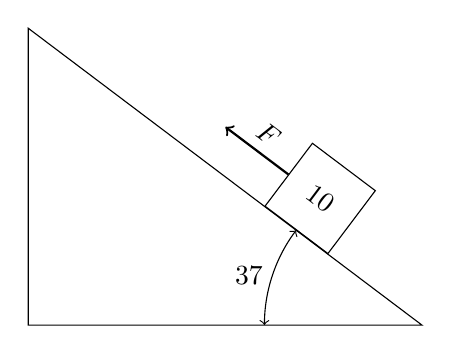
\begin{tikzpicture}
        %% Incline
        \draw (0,0) -- (-5,3.77) -- (-5,0) -- cycle;
        \draw[<->] (0,0) ++ (180:2) arc (180:143:2) node[pos=0.5,anchor=east] {\ang{37}};
        %% Mass
        \node[rotate=-37,draw,minimum size=1cm,anchor=south] (M) at (143:2) {\SI{10}{\kilo\gram}};
        %% Force
        \draw[thick,->] (M.west) -- ++(143:1) node[pos=0.5,anchor=south,rotate=-37] {$F$};
    \end{tikzpicture}
    \end{center}
    The coefficient of kinetic friction between the block and the inclined surface is \num{0.2}.
    \begin{multicols}{3}
    \begin{choices}
      \correctchoice{\SI{76}{\newton}}
        \wrongchoice{\SI{54}{\newton}}
        \wrongchoice{\SI{42}{\newton}}
        \wrongchoice{\SI{36}{\newton}}
        \wrongchoice{\SI{28}{\newton}}
    \end{choices}
    \end{multicols}
\end{question}
}

\element{njctl}{
\begin{question}{dynamics-q31}
    A sphere of mass $m$ falls in the presence of air resistance.
    If the air resistance force is given $F=-bv$ and at time $t=0$, $v_0=0$,
        which of the following expressions is the velocity of the sphere as a function of time?
    \begin{multicols}{2}
    \begin{choices}
      \correctchoice{$v = \dfrac{mg}{b}\left(1-\mathrm{e}^{-\dfrac{bt}{m}}\right)$}
        \wrongchoice{$v = \dfrac{m}{b}\left(1-\mathrm{e}^{-\dfrac{bt}{m}}\right)$}
        \wrongchoice{$v = \dfrac{g}{b}\left(1-\mathrm{e}^{-\dfrac{bt}{m}}\right)$}
        \wrongchoice{$v = \dfrac{b}{mg}\left(1-\mathrm{e}^{-\dfrac{bt}{m}}\right)$}
        \wrongchoice{$v = \dfrac{mg}{b}\left(1-\mathrm{e}^{-\dfrac{mt}{b}}\right)$}
        %% \left \right)
        %\correctchoice{$v = \dfrac{mg}{b}\left(1-\mathrm{e}^{-\left(\dfrac{bt}{m}\right)}\right)$}
        %\wrongchoice{$v = \dfrac{m}{b}\left(1-\mathrm{e}^{-\left(\dfrac{bt}{m}\right)}\right)$}
        %\wrongchoice{$v = \dfrac{g}{b}\left(1-\mathrm{e}^{-\left(\dfrac{bt}{m}\right)}\right)$}
        %\wrongchoice{$v = \dfrac{b}{mg}\left(1-\mathrm{e}^{-\left(\dfrac{bt}{m}\right)}\right)$}
        %\wrongchoice{$v = \dfrac{mg}{b}\left(1-\mathrm{e}^{-\left(\dfrac{mt}{b}\right)}\right)$}
        %% exp(
        %\correctchoice{$v = \dfrac{mg}{b}\left(1-\mathrm{e}^{-\dfrac{bt}{m}}\right)$}
        %\wrongchoice{$v = \dfrac{m}{b}\left(1-\mathrm{e}^{-\dfrac{bt}{m}}\right)$}
        %\wrongchoice{$v = \dfrac{g}{b}\left(1-\mathrm{e}^{-\dfrac{bt}{m}}\right)$}
        %\wrongchoice{$v = \dfrac{b}{mg}\left(1-\mathrm{e}^{-\dfrac{bt}{m}}\right)$}
        %\wrongchoice{$v = \dfrac{mg}{b}\left(1-\mathrm{e}^{-\dfrac{mt}{b}}\right)$}
    \end{choices}
    \end{multicols}
\end{question}
}

\element{njctl}{
\begin{question}{dynamics-q32}
    In the physics lab,
        a student performs an experiment with a double-sided spring gun.
    When the spring is compressed and then released it can fire two rubber balls $m_1$ and $m_2$ at the same time.
    \begin{center}
    \begin{tikzpicture}
    \end{tikzpicture}
    \end{center}
    From this experiment the student was able to measure only the acceleration of each ball $a_1$ and $a_2$.
    Based on this information,
        which of the following can be determined?
    \begin{choices}
        \wrongchoice{$m_1$ and $m_2$ only}
        \wrongchoice{Spring force $F$ only}
        \wrongchoice{Spring force $F$, $m_1$ and $m_2$}
      \correctchoice{Ratio of $m_1$ and $m_2$ only}
        \wrongchoice{Ratio of $m_1$ and $m_2$ , and spring force $F$ only}
    \end{choices}
\end{question}
}

\newcommand{\njctlDynamicsQThirtyThree}[1]{
\begin{tikzpicture}
    %% Incline
    \draw (0,0) -- (-4.33,2.5) -- (-4.33,0) -- cycle;
    \draw[<->] (0,0) ++ (180:1.5) arc (180:150:1.5) node[pos=0.5,anchor=east] {$\theta$};
    %% Mass
    \node[rotate=-30,draw,minimum size=0.7cm,anchor=south] (M) at (150:3) {$m$};
    %% Force
    \draw[thick,->] (M.east) -- ++(330:1) node[pos=0.5,anchor=south,rotate=-30] {$#1$};
\end{tikzpicture}
}

\element{njctl}{
\begin{question}{dynamics-q33}
    A block of mass $m$ moves with acceleration, $a$, down a frictionless inclined plane that makes an angle $\theta$ with the horizontal.
    \begin{center}
        \njctlDynamicsQThirtyThree{a}
    \end{center}
    Which of the following expressions about the normal force on the block is correct?
    \begin{multicols}{2}
    \begin{choices}
        \wrongchoice{$F_n = mg$}
        \wrongchoice{$F_n = mg\sin\theta$}
      \correctchoice{$F_n = mg\cos\theta$}
        \wrongchoice{$F_n = ma$}
        \wrongchoice{$F_n = mg\tan\theta$}
    \end{choices}
    \end{multicols}
\end{question}
}

\element{njctl}{
\begin{question}{dynamics-q34}
    A block of mass $m$ moves with acceleration, $a$, down a frictionless inclined plane that makes an angle $\theta$ with the horizontal.
    \begin{center}
        \njctlDynamicsQThirtyThree{a}
    \end{center}
    Which of the following expressions about the acceleration of the block is correct?
    \begin{multicols}{2}
    \begin{choices}
        \wrongchoice{$a = g$}
      \correctchoice{$a = g\sin\theta$}
        \wrongchoice{$a = g\cos\theta$}
        \wrongchoice{$a = 2g$}
        \wrongchoice{$a = g\tan\theta$}
    \end{choices}
    \end{multicols}
\end{question}
}

\element{njctl}{
\begin{question}{dynamics-q35}
    A block slides at a constant velocity down the inclined plane that makes an angle $\theta$ with the horizontal.
    \begin{center}
        \njctlDynamicsQThirtyThree{v}
    \end{center}
    Which of the following expressions represents the coefficient of kinetic friction between the block and the inclined surface?
    \begin{multicols}{3}
    \begin{choices}
      \correctchoice{$\tan\theta$}
        \wrongchoice{$\sin\theta$}
        \wrongchoice{$\cos\theta$}
        \wrongchoice{$\dfrac{1}{\tan\theta}$}
        \wrongchoice{$\dfrac{1}{\sin\theta}$}
    \end{choices}
    \end{multicols}
\end{question}
}

\element{njctl}{
\begin{question}{dynamics-q36}
    An object of mass \SI{1}{\kilo\gram} starts from rest and moves along a straight line.
    The velocity as a function of time is given $v = 3t^2 + 2t$,
        where all values are in base SI units.
    What is the instantaneous force on the object at time $t = \SI{3}{\second}$?
    \begin{multicols}{3}
    \begin{choices}
        \wrongchoice{\SI{10}{\newton}}
      \correctchoice{\SI{20}{\newton}}
        \wrongchoice{\SI{30}{\newton}}
        \wrongchoice{\SI{40}{\newton}}
        \wrongchoice{\SI{50}{\newton}}
    \end{choices}
    \end{multicols}
\end{question}
}

\element{njctl}{
\begin{question}{dynamics-q37}
    A \SI{10}{\kilo\gram} box is pushed with an initial velocity of \SI{4}{\meter\per\second} on a horizontal surface.
    The box moves \SI{8}{\meter} before it comes to a complete stop.
    What is the coefficient of kinetic friction between the box and the surface?
    \begin{multicols}{3}
    \begin{choices}
        \wrongchoice{\num{0.30}}
        \wrongchoice{\num{0.20}}
      \correctchoice{\num{0.10}}
        \wrongchoice{\num{0.05}}
        \wrongchoice{\num{0.02}}
    \end{choices}
    \end{multicols}
\end{question}
}

\newcommand{\njctlDynamicsQThirtyEight}{
\begin{tikzpicture}
    %% NOTE: tikz
    %% Ground
    \draw (-3,0) -- (3,0);
    \node[anchor=north,fill,pattern=north east lines,minimum width=6cm, minimum height=0.05cm] at (0,0) {};
    %% masse
    \node[draw,minimum width=3cm,minimum height=1cm,rounded corners=0.5ex,anchor=south] (A) at (0,0) {\SI{20}{\kilo\gram}};
    \node[draw,minimum width=1.7cm,minimum height=0.71cm,rounded corners=0.5ex,anchor=south] (B) at (A.north) {\SI{10}{\kilo\gram}};
    %% force
    \draw[thick,->] (A.east) -- ++(0:2) node[pos=0.5,anchor=south] {$F=\SI{150}{\newton}$};
\end{tikzpicture}
}

%% NOTE: question idea: have F large enough to cause top to slide
\element{njctl}{
\begin{question}{dynamics-q38}
    A \SI{10}{\kilo\gram} block is place on top of the \SI{20}{\kilo\gram} block as shown.
    The system of two blocks can move on a horizontal frictionless surface.
    The coefficient of static friction between the blocks is \num{0.6}.
    \begin{center}
        \njctlDynamicsQThirtyEight
    \end{center}
    If a horizontal \SI{150}{\newton} force is applied to the \SI{20}{\kilo\gram} block and the top block doesn't slide on the bottom block,
        what is the acceleration of the system?
    \begin{multicols}{3}
    \begin{choices}
        \wrongchoice{\SI{1}{\meter\per\second\squared}}
        \wrongchoice{\SI{3}{\meter\per\second\squared}}
      \correctchoice{\SI{5}{\meter\per\second\squared}}
        \wrongchoice{\SI{7}{\meter\per\second\squared}}
        \wrongchoice{\SI{9}{\meter\per\second\squared}}
    \end{choices}
    \end{multicols}
\end{question}
}

\element{njctl}{
\begin{question}{dynamics-q39}
    A \SI{10}{\kilo\gram} block is place on top of the \SI{20}{\kilo\gram} block as shown.
    The system of two blocks can move on a horizontal frictionless surface.
    The coefficient of static friction between the blocks is \num{0.6}.
    \begin{center}
        \njctlDynamicsQThirtyEight
    \end{center}
    If a horizontal \SI{150}{\newton} force is applied to the \SI{20}{\kilo\gram} block and the top block doesn't slide on the bottom block,
        what is the magnitude of the horizontal force that the \SI{10}{\kilo\gram} block exerts on the \SI{20}{\kilo\gram} block?
    \begin{multicols}{3}
    \begin{choices}
        \wrongchoice{\SI{10}{\newton}}
        \wrongchoice{\SI{20}{\newton}}
        \wrongchoice{\SI{30}{\newton}}
      \correctchoice{\SI{50}{\newton}}
        \wrongchoice{\SI{60}{\newton}}
    \end{choices}
    \end{multicols}
\end{question}
}

\element{njctl}{
\begin{question}{dynamics-q40}
    A block is given an initial velocity $v_0$ when it is at the bottom of a rough inclined plane.
    \begin{center}
    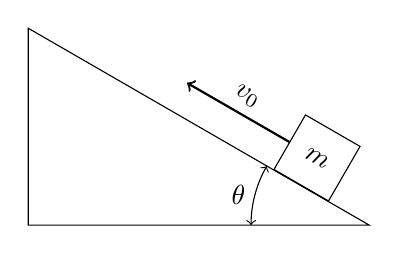
\begin{tikzpicture}
        %% Incline
        \draw (0,0) -- (-4.33,2.5) -- (-4.33,0) -- cycle;
        \draw[<->] (0,0) ++ (180:1.5) arc (180:150:1.5) node[pos=0.5,anchor=east] {$\theta$};
        %% Mass
        \node[rotate=-30,draw,minimum size=0.8cm,anchor=south] (M) at (150:1) {$m$};
        %% Force
        \draw[thick,->] (M.west) -- ++(150:1.5) node[pos=0.5,anchor=south,rotate=-30] {$v_0$};
    \end{tikzpicture}
    \end{center}
    Which of the following is true about the block as it moves?
    \begin{choices}
        \wrongchoice{It has the same acceleration as it moves up and down the plane.}
      \correctchoice{It has greater acceleration as it moves up the plane and less acceleration as it moves down the plane.}
        \wrongchoice{It has greater acceleration as it moves down the plane and less acceleration as it moves up the plane.}
        \wrongchoice{It has a varying acceleration as it moves up and down the plane.}
        \wrongchoice{It has a constant velocity as it moves up and down the plane}
    \end{choices}
\end{question}
}

%% ANSWERS:
%% 1.C 2.C 3.C 4.D 5.D 6.C 7.B 8.A 9.C 10.C 11.A 12.D 13.B 14.B 15.A 16.C 17.C 18.E 19.D 20.E 21.A 22.E 23.B 24.C 25.D 26.B 27.A 28.E 29.E 30.A 31.A 32.D 33.C 34.B 35.A 36.B 37.C 38.C 39.D 40.B

\endinput


